\documentclass[PICOReport.tex]{subfiles}

%\newcolumntype{L}[1]{>{\raggedright\let\newline\\\arraybackslash\hspace{0pt}}m{#1}}
%\newcolumntype{K}[1]{>{\raggedright\centering\arraybackslash}m{#1}}

\begin{document}

Having flown two space missions (WMAP and \planck ) and fielded numerous sub-orbital experiments to measure polarization, the mm/sub-mm wavelength community has gained extensive experience with systematic uncertainties that occur in various experimental configurations. 
A rich literature investigates the types of systematic errors due to the environment, the instrumentation, observation strategies, and data analysis that could confound polarization measurements by creating a bias or an increased variance \cite{hu03,shimon2008,yadav2010,Griffiths2014,LFI_systematics,Kaplan2002,Miller2009,Pagano2009,SO_sys_optical,SO_sys_detector, bicep_systematics,SPIDER_systematics}. Teams have used the accumulated experience to incorporate technological solutions during the design phase, and to optimize data analysis techniques to identify and compensate for systematic errors. 
%As a consequence, all of the cosmological results reported to date are noise, not systematic uncertainty limited. In several cases systematic effects have been identified in the data, but then suppressed to levels below the noise. 

Just as requirements on signal separation (\S~\ref{sec:signal_separation}) are determined by the need to reach the faintest inflationary signal, so are the requirements on control of systematic uncertainties. Since an inflationary $BB$ power spectrum with $r = 5 \times 10^{-4}$ has a peak signal level of 7~nK, systematic effects need to be controlled to a level of $\sim$1~nK. It has long been recognized that exquisite control of systematic uncertainties will be required from any experiment attempting to reach levels of $r \lesssim 1\times 10^{-3}$, and it is widely accepted that the stability provided aboard a space platform makes it best suited to control systematic uncertainties compared to other platforms. This is one of the most compelling reasons to observe from space.  As WMAP and \planck~ demonstrated, an L2 orbit offers excellent thermal stability, as well as flexibility in the choice of scan strategy.  

Sources of systematic effects and their ultimate degree of severity are a function of the instrument implementation, the spacecraft scan strategy, and mitigations methods developed during the data analysis pipeline. Thus, a proper assessment requires end-to-end simulation of the mission. Such a simulation should include realistic instabilities and non-idealities of the spacecraft, telescope, and instrument, as well as folding in data post-processing techniques. Developing such a simulation is a significant undertaking, which took years  for the \planck\ mission, and was beyond the scope of this study. We have instead opted to (1)~implement design features within PICO that would provide strong data redundancy and enable cross-checks during the data analysis~(\S~\ref{sec:systematics_key}), and (2)~enumerate the sources of possible systematic errors, assess their effects, and investigate three that were deemed the highest priority~(\S~\ref{sec:systematics_list}--\S~\ref{sec:fsl}). 

%PICO takes advantage of an L2 orbit, using a rotating spacecraft (at 1~rpm) whose spin axis precesses with a 10~hour period, thus scanning the sky in a way that is crosslinked on many time scales and at many angles, without interference from the Sun, Earth, or Moon; this reduces the effects of low frequency noise without the need for additional internal-to-the-instrument mechanical modulation. The redundancy of observations allows the checking of consistency of results and an improved ability to calibrate and to correct systematic errors in post-processing analysis.\comor{should we say it here or in the end?}

% redundancy: 13,000 independent q,u,i maps; 10 independent surveys maps of the sky
%We expect the following paradigm to continue: if a systematic effect is large enough to exist above the noise level, it can be characterized and suppressed. 

%In the near term, the ground-based and suborbital CMB community will continue to develop new techniques in handling systematics, particularly in developing the CMB-S4 project.

%As an example, BICEP systematics limited it to r=0.1\cite{Takahashi2010} while through additional effort within the program, BICEP2 achieved a systematics limit of r=6$\times$10$^{-3}$\cite{BICEP2_III}). In the near term, the ground-based and suborbital CMB community will continue to develop new techniques in handling systematics, particularly in developing the CMB-S4 project.

%All prior on-orbit measurements of CMB polarization were limited by systematic errors until an in-depth study of the systematics was performed allowing a post-processing data analysis to suppress them \cite{Bennett13,planck2016_xlvi,Planck2018_I}. Particularly we note figure 3 of Ref.\cite{Planck2018_I} which quantifies \planck's systematic error limits on the polarization power spectral measurements. Recently studied space missions, such as EPIC-IM, LiteBird and  \core, have placed systematic error mitigation at the forefront of the case for their mission and have developed tools and strategies for estimating and mitigating these\cite{hazumi2012,wallis2017,Natoli2018}.

\subsubsection{Potential Systematics Effects}
\label{sec:systematics_list}


The systematic effects faced by PICO can be grouped into three broad categories: (1)~Coupling between signals; (2)~stability; and (3)~stray light. For the first category, the most important are the intensity coupling into polarization (both $E$ and $B$) and $E$ coupling into $B$. This is because $T$ (denoting intensity) is approximately ten times stronger than $E$, which is approximately ten times stronger than $B$. The systematic effects are listed in Table \ref{tbl:SystematicsList2col} and were prioritized for further study using a priority factor incorporating a PICO Systematics Working Group's assessment of how mission-limiting the effect is, how well these effects are understood by the community and whether mitigation techniques exist.  

We used simulations to investigate the following three effects that had the highest priority: error in the absolute calibration of polarization angle; error in the relative calibration between orthogonally oriented detectors, and the effect of the telescope sidelobes. We adapted tools developed for \planck~\cite{plank2015_xii_focalplane} and in the context of a European-led mission concept~\citep{core_systematics}. To understand the severity of the effects, we analyzed each in isolation, and in most cases without complicating effects such as inclusion of foreground-separation steps. More detailed studies of the combination of effects and the inclusion of a foreground-separation step are important but are left to the future. 

%We note that many of the systematics could be mitigated further through the use of polarization modulation such as a half-wave plate or a variable phase delay modulator.  
%For the purposes of the cost constraints of PICO, we investigated mitigation techniques that do not require a modulator.  

%\input tables/table2.2.tex
\input tables/table2.2_wide.tex


\subsubsection{Absolute Polarization Angle Calibration}
\label{sec:angle}

In PICO, each of the Stokes $Q$ and $U$ parameters along any line of sight is evaluated through having sensitivity to two orthogonal polarization states. The relative designation of $Q$ and $U$ is derived from having sensitivity to pairs of polarization orientations that are 45\degree\ apart. A systematic error in the implementation (or estimation) of these angles by an amount $\alpha$ causes signals in $Q$ and $U$, and thus in $E$ and $B$ to mix. Because the CMB $E$ is much larger than $B$, mixing between $E$ and $B$ leads to the generation of a spurious $BB$ angular power spectrum that mirrors the shape of the $EE$ spectrum~(Fig.~\ref{fig:rot_bb_tb_eb}). The level of spurious $BB$ is proportional to $\alpha^{2} \times EE$. At angular multipoles $\ell \lesssim 100$ a systematic error $\alpha\approx 10\arcmin$ will result in a spurious $BB$ level that is approximately equivalent to $r \sim 1\times10^{-4}$~\citep{shimon2008,Aumont+2018}.  The mixing of $E$ and $B$ also leads to spurious cross-spectra $EB$ and $TB$, that respectively mimic the $EE$ and $TE$ spectra. 

The systematic error is most usefully split to two contributions: an overall `absolute' error in the assumed instrument's sensitivity to polarization orientations relative to fixed sky coordinates, and a `relative' rotation error between various pairs of detectors. For PICO, the relative rotation of the detectors will be measured to $\sim 0.1\arcmin$ by comparing the measured polarization signals between many independent detectors and pairs. However, directly measuring the overall rotation in flight -- which is the process of calibrating the polarization angles --  is challenging as there are no sufficiently well calibrated polarized astronomical sources. For example, \citet{Aumont+2018} showed that the current uncertainty of $0.33$\degree\ on the Crab polarization orientation limits measurements to $r \sim 0.01$, which is much larger than PICO's target. 

PICO will overcome this potential source of error through using its high \ac{SNR} measurement of the polarization to identify and reduce it below relevant levels in data analysis. \citet{yadav2010} showed that because the $T$ and $E$ signals are much stronger than $B$, an experiment that searches for a specific level of cosmological $BB$ will have high \ac{SNR} for detecting the spurious $EB$ and $TB$ cross-spectra. Applying their method to the PICO baseline specifications we find that with PICO we will constrain overall rotation to a level of $\alpha=0.2\arcmin$ and $0.6\arcmin$ $(3\sigma)$ using the $EB$ and $TB$ spectra, respectively, suppressing this systematic effect to negligible levels~(Fig.~\ref{fig:rot_bb_tb_eb}). The constraints quoted include delensing level of 73\%, which is the PICO forecast including foreground separation. 


%The measured CMB polarization can be rotated due to (1) a birefringent primordial Universe, or a Faraday rotation due a primordial magnetic field \citep{Pogosian+2018}; (2) birefringent foregrounds, or interaction with the Galactic magnetic field; (3) systematic effects in the instrument, and in particular an error in the direction of polarization measured by each detector.   While the first two sources create a rotation that may depend on scale, position and/or frequency, the latter depends mainly on the detector itself. 

%A rotation {\prang} of the direction of polarization mixes the $Q$ and $U$ Stokes parameters via $Q\pm iU \longrightarrow e^{\mp i 2 \prang} (Q\pm iU)$ and thus mixes the power spectra and their correlations, as illustrated in Fig.~\ref{fig:rot_bb_tb_eb}.


%------------------------------------------------------------------------------------------

%The most recent constraints on cosmological birefringence \citep{Planck2016_XLIX} were limited by uncertainties on the detector orientations.  In \planck, the detectors were characterized pre-launch to $\pm 0.9^\circ$ (rel.) $\pm 0.3^\circ$ (abs.) \citep{Rosset+2010}. For \pico, the relative rotation of the detectors will be measured to a few $0.1\arcmin$ using the CMB, but the overall rotation is unlikely to be known pre-launch to better than \planck.  Known polarized sources, such as the Crab Nebula, are not characterized well enough independently to serve as calibrators; \citet{Aumont+2018} show that the current uncertainty of $0.33^\circ$ on the Crab polarization orientation, limits a $B$-mode measurement to $r \sim 0.01$, far from \pico's target.

%Figures \ref{fig:rot_sens_0} and \ref{fig:rot_sens_2} show how the measurement of $r$ by \pico\ is degraded because of an overall rotation of polarization, and how $TB$ and $EB$ can be used to monitor this rotation, assuming that the only source of polarization rotation is instrumental.
%These results are obtained assuming the spectra to have a Gaussian likelihood, with a variance $\propto 1/\fsky$, and ignoring the foreground contributions.

\subsubsection{Differential Gain}
\label{sec:gain_stability}

Photometric calibration is the process of converting the raw output of each detector -- typically given in digital detector readout units -- to physical units via a calibration factor $C(t)$, which is a function of time. One straightforward way for PICO to derive $Q$ and $U$ is through differencing detectors that are sensitive to two orthogonal polarization states $A$ and $B$. A systematic error in the determination of either of the $A$ or $B$ calibration factors will translate to a biased $Q$ or $U$. We investigated whether the anticipated error on $C_{A,B} (t)$ is adequate for PICO's requirements on measuring the faint inflationary signal.  
%However, statistical or systematic errors in the determination of $G_{A}(t)$ and $G_{B}(t)$ translate to increased uncertainties, or biased results, respectively.  We investigated whether the anticipated error on $G(t)$ is adequate for PICO's requirements on measuring the faint inflationary signal.  

The inflationary signal will be extracted from data in the primary CMB bands between 60 and 300~GHz. Detectors in these bands will be calibrated using measurements of the CMB dipole, a signal that will be measured once per minute as the telescope scans the sky (\S~\ref{sec:survey_design}).  We evaluated the combined impact of the scan strategy and white- and 1/f-noise in the estimation of $C(t)$.
%\footnote{We use software tools developed for and validated in the context of analysis of the \planck/LFI data.} 
The simulation included signals from the anisotropy of the CMB, including the dipole and $BB$ lensing. Full details of the simulation pipeline are available in the PICO website~\citep{picoweb_simulating}. Fig.~\ref{fig:rot_bb_tb_eb} demonstrates that the power spectrum due to error in $C_{A,B} (T)$ is much lower than the PICO requirement of $\sigma(r) = 1\times 10^{-4}$. 
\begin{figure}[thb]
\centerline{
\includegraphics[width=0.375\textwidth]{images/PICO_rotate_eb6_v3.\suffix} 
\hspace{0.3in}
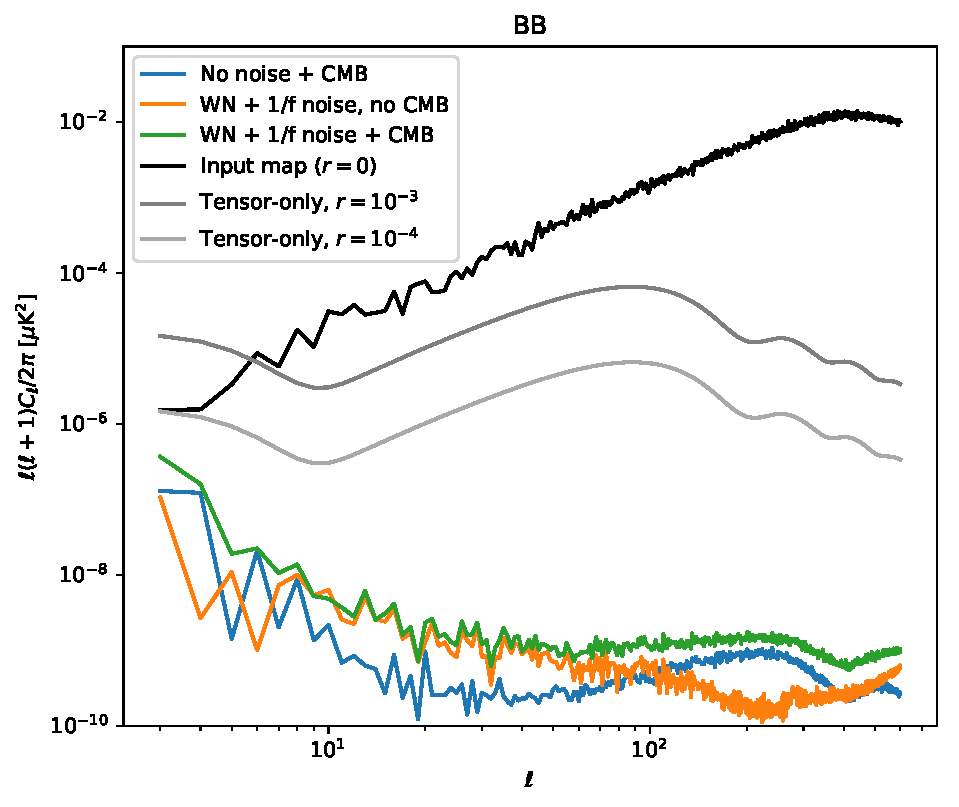
\includegraphics[width=0.41\textwidth]{images/calibration_spectrum_BB.pdf} }
\vspace{-0.1in}
\caption{\captiontext
Two of the initially-estimated highest priority systematic effects for PICO can be suppressed to low levels relative to requirements; we show inflationary signals with  $r = 1\times 10^{-4}\,\, \mbox{and} \,\, 1\times 10^{-3}$ (solid and dash orange, respectively), and $BB$ lensing (black, theory on the left; realization on right). Left: The residual spurious $BB$ spectrum due to 0.2\arcmin\ mis-calibration of PICO's angles of polarization sensitivity (solid blue) has the shape of the $EE$ spectrum, and is small compared to the requirement for $\ell<200$ and compared to the baseline statistical noise level (grey dash). Right: simulated residual $BB$ power after accounting for calibration drifts (solid blue). 
\label{fig:rot_bb_tb_eb} }
\vspace{-0.1in}
\end{figure}

%A more complete data-analysis pipeline would pair the calibration step with the component-separation step, following a scheme similar to \planck/LFI's final data processing \cite{Planck2018_II}: the calibration code is followed by a component-separation analysis, and these two steps are iterated until the solution converges. 

%We simulated the time stream signals of four detectors over the duration of the mission, including PICO baseline noise levels, 1/f noise parameters, and the scan strategy. We solved (\S~\ref{sec:??}) \comor{where?}. We fit the  an end-to-end simulation using

%instrument and the CORE mission proposal. The quality of the estimate depends on the noise level of the receivers, but also on the details of the scanning strategy.  To analyze the impact of calibration uncertainties on PICO, we performed  the following analysis. Firstly, we simulated the observation of the sky, assuming four receivers, the nominal scanning strategy, and $1/f$ noise. The simulated sky contained CMB anisotropies, plus the CMB dipole. Then we ran the calibration code to fit the dipole against the raw data simulated during the first step. We again simulated the observation of the sky, this time using the values of $G$ computed during the second step, which contain errors due to the presence of noise and the CMB signal.

%Results of the simulation (neglecting foregrounds) are shown as power spectrum residuals in Fig.~\ref{fig:rot_bb_tb_eb}. We estimate the gain fluctuations to better than 10$^{-4}$ when solving for the gain every 40 hours (4 precession periods). The scanning strategy employed by PICO allows for a much better calibration than was possible for \planck, thanks to the much faster precession.

\subsubsection{Far Sidelobes}
\label{sec:fsl}
%The main beam (within a few degrees of the axis of beam response) in a CMB mission can be measured to high precision using the planets .  

Differences between the assumed and actual antenna pattern of the detectors will give rise to systematic errors. \planck 's ground-based measurements mapped the antenna response to levels down to $-90$~dB from the main lobe \comor{give range from Karl}. The best in-flight measurements, made through repeated passes of solar system planets reached levels of $-60$~dB~\citep{tauber2018}. Thus in-flight measurements were only useful to reconstruct in-flight antenna pattern within a region of few degrees of the main lobe, not in the `far sidelobes' of the antenna response.  

Far-sidelobe response can couple to bright Galactic signals when the telescope points tens of degrees away from the Galactic plane. If such far-sidelobe response is not known, the signals could be interpreted as faint cosmological signals and bias estimates of their magnitude. To evaluate PICO's susceptibility to this systematic effect we used the same physical optics software as used by \planck\ to compute PICO's $4\pi$~sr antenna response for four 155~GHz detectors located at the center of the focal plane. We simulated the time domain response of the detectors as they scanned the sky over a year of PICO observations. We convolved their antenna response with a full-sky Galactic emission model~\citep{thorne2018_pysm}, reconstructed maps of $I$, $Q$, and $U$, and calculated the resulting $BB$ angular power spectrum when using a \planck\ Galactic mask excluding 60\% of sky~\citep{planck_2013_xv}. 

The largest sidelobe in the antenna response is at a level of $-80$~dB from the main lobe. We find that if that sidelobe is known with \ac{SNR} of \comred{20}, or further suppressed by that factor, the contamination from the sidelobe is suppressed to more than a factor of ten below the requirement of $\sigma(r) = 5 \times 10^{-4}$. This suppression can be achieved by adjusting the instrument design, e.g. adding baffles, or by modeling, measuring, and removing the sidelobe pickup during data analysis. 


 
%Measurement of each detector's response to signals off axis, which tends to be weak (--80dB less than the peak response) but spread over a very large solid angle, is difficult to do pre-launch, and may not even be done accurately after launch.  Nonetheless, this far sidelobe can couple bright Galactic signals from many tens of degrees off-axis and confuse it with polarized signal from the CMB off the Galactic plane.    To evaluate this systematic error, GRASP software was used to compute the PICO telescope's response over the full sky.  The computed full-sky beams showed features peaking at about -80\,dB of the on-axis beam.   


\subsubsection{Key Findings}
\label{sec:systematics_key}

Properly modeling, engineering for, and controlling systematic effects are key for the success for any experimental endeavor striving to achieve $\sigma(r) \lesssim 1 \times 10^{-4}$. Based on extensive community experience with both hardware and analysis of data collected in space and in sub-orbital experiments we note the following points: \\
$\bullet$ \hspace{0.1in}  Relative to other platforms, a space-based mission provides the most thermally stable platform, and thus the pre-requisite for improved control of systematic effects. PICO's orbit at $L2$ is among the most thermally stable of possible orbits. \\
$\bullet$ \hspace{0.1in} PICO's sky scan pattern will give strong data redundancy, which will enable numerous cross-checks. Each of the 12,996 detectors will make independent maps of the $I,\,Q$, and $U$ Stokes parameters enabling many comparisons within and across frequency bands, within and across sections of the focal plane, and within and across bolometers that have the same (or different) polarization sensitivities. Half the sky is scanned every two weeks, and the entire sky is scanned in 6 months. Thus combinations of maps constructed at different times during of the mission will be differenced to search for residual time-dependent systematic effects. \\
$\bullet$ \hspace{0.1in}  The PICO scan pattern gives almost continuous scans of planets; \planck\ observed each of the planets with a 6 month cadence. This will significantly improve antenna pattern characterization. The scan pattern also has the benefit of nearly continuous large-amplitude CMB dipole signals, which will give high \ac{SNR} calibration. \\
$\bullet$ \hspace{0.1in}  We showed that two of the highest priority factor systematic effects can be controlled to levels that are small compared to requirements. More analysis and planning is required to address systematic uncertainties arising from the far sidelobe response of the telescope. 

Undoubtedly, more work is required to analyze other systematic effects, their combination, and their coupling with foreground separation. We strongly recommend that support be provided for such activities. Specifically, support for suborbital efforts is essential to continue the development of means to identify systematic effects, and to develop new techniques to mitigate them. In addition, we endorse support for the development of a complete end-to-end software simulation facility, which is the only to quantify mission trade-offs under the influence of a combination of systematic effects that are coupled to the task of signal separation.  

%\comred{Previous Text}

%\comor{As of today, we conclude that there is a clear path to demonstrate that state-of-the-art technology and data processing can take advantage of the L2 environment and control systematic errors to a level that enables the science goals of PICO. In particular we note the following points:
%\begin{itemize}
%\item The raw sensitivity of the instrument should include enough margin that data subsets can independently achieve the science goals. This allows testing of the results in the data analysis and additional data cuts, if needed.
%\item For PICO mission, a physical optics model of the telescope should be developed, enabling full-sky beam calculations, which should be validated as much as possible on the ground.  This will be needed to characterize and remove far-sidelobe pickup seen during the mission. 
%\item NASA's support of ground-based and suborbital CMB missions will mitigate risk to a future space mission such as PICO by continuing to develop analysis techniques and technology for the reduction of systematic errors.
%\item In the PICO mission's Phase~A, a complete end-to-end system-level simulation software facility should be developed to assist the team in setting requirements and conducting trade-offs between subsystem requirements while realistically accounting for post-processing mitigation.  Any future CMB mission is likely to have similar orbit  and scan characteristics to those of PICO, thus there is an opportunity for NASA and the CMB community to invest in further development of this capability now.
%\item Low frequency excess noise (also called 1/f noise) should be studied in detail as part of a simulation effort to set detailed detector and systems level requirements.  The systematics simulations performed here show that PICO's science goals can be achieved with no additional modulation and assuming current state-of-the-art levels of low frequency noise (a total knee frequency of 20~mHz) based on demonstrated TES performance, and system-level residuals achieved by \planck.
%\end{itemize} }


\end{document}


